\documentclass[a4paper, 12pt, finnish]{report}
\usepackage[utf8]{inputenc}
\usepackage{amsfonts}
\usepackage{graphics}
\usepackage[finnish]{babel}
\usepackage{titlesec}
\titleformat{\chapter}
{\Large\bfseries}
{}            
{0pt}      
{\huge} 

\newcommand{\topic}{My application the chairperson of the represetantive council}
\usepackage{hyperref}
\hypersetup{pdfpagemode=UseNone, pdfstartview=FitH, colorlinks=true,urlcolor=red,linkcolor=blue,citecolor=black,pdftitle={\topic},pdfauthor={Onni Lampi}}
\setlength{\parindent}{0mm}
\setlength{\emergencystretch}{15pt}
\newcommand*{\findate}{\the\day.\the\month.\the\year}

\begin{document}



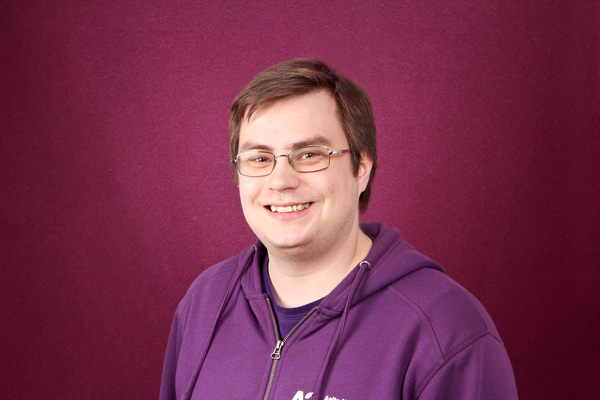
\includegraphics{onnilampi_ayy.jpg}
\section*{\topic}


I'm Onni, 25 years old communications technology student from ELEC.
During my studies in Aalto, AYY has grown to be a very dear organization for me.
This year almost all of my time has been allocated to being a member of the AYY board.
Seeing the student unions functions so closely for an entire year made me want to contribute more, so decided to apply for the chair of the represetantive council, in order to enable the councils decision making on a more conrete level. \\


As a person I'm calm, diligent and I have a somewhat unique sense of humor.
I take great pride in doing my job as carefully and steadily as possible, I don't like to rush things.
Sometimes quick decisions are necessary, and I'm good at doing them because of my earlier experience in rather hectic positions.\\

The represetantive council is very important to me.
All the most crucial decisions and values are done by the council, and I want to be a part of this process next year.
Next year the council will work on the strategy of the student union for the coming years.
In addition, numerous policy papers and regulations are under updates and additions, some might not materialize for years.
This means, that a huge amount of dialogue and discussion is needed between the council and the student unions board.
Because of these reasons the role of chair and vice chairs in the process is greatly emphasized!\\

This year, first real trials with Council Committees have been carried out with great success!
I plan to continue working closely with the chairpersons of the Committees in co-operation with the AYY board.
It is also important to elect the Committees so that all the council groups are reprecented fairly.\\

One should not forget the before mentioned council groups!
The groups form the spine of the represetantive council, so they need to be assisted in any means necessary.
I'd like to see one of the vice chairs to take that burden to their behalf, so that we can be sure that the resources are sufficient.
The another vice chair could for example take care of the trilinguality of the council.
To me it is important to take it seriously, so that the entire community can take part in the discussion.\\

The most important job of the Council Chair is to enable efficient function in the council.
In my opinion I would be the right person for the job, and I'd like to make this year the best one yet!\\

Regards, Onni


\subsection*{Please ask more from me!}
Onni Lampi\\
040 702 3841\\
omnez@telegram\\
contact@onnilampi.fi

\end{document}

